\documentclass[../root.tex]{subfiles}

\begin{document}
\section{Examples} \label{sec:mpc_examples}
The following examples were run on an Intel i7-1165G7 processor. For the QP
examples, ALTRO-C was compared against OSQP \cite{stellato_OSQP_2020}, a
state-of-the-art ADMM QP solver optimized for online optimization, and the
SOCP examples were compared against ECOS \cite{domahidi_ECOS_2013}, an
interior-point SOCP solver designed for embedded applications, COSMO
\cite{garstka_COSMO_2019}, a state-of-the-art ADMM SOCP method, and
Mosek\footnote{\url{https://www.mosek.com/}}, a high-quality commercial
convex optimization package. All problems were solved to cost and constraint
tolerances of $10^{-4}$, so the solution-polishing steps of both ALTRO-C and
OSQP were disabled. The reported timing results only capture the time to
solve the convex optimization problem: All overhead associated with modifying
the problem during each MPC iteration is omitted. Future work with emphasis
on applications will include the often non-trivial steps required to
efficiently update the problem between iterations, although fast and
allocation-free methods are already implemented in ALTRO-C\footnote{Available
in the \href{https://github.com/RoboticExplorationLab/Altro.jl}{Altro.jl} and
\href{https://github.com/RoboticExplorationLab/TrajectoryOptimization.jl}{TrajectoryOptimization.jl}
packages}. Code for the examples is available at
\url{https://github.com/RoboticExplorationLab/altro-mpc-icra2021}.

\subsection{Random Linear MPC}
We compared the general performance of ALTRO-C and OSQP on a set of random
QPs of the following form:
\begin{mini}[2] 
    {X,U}{\sum_{k=1}^N \norm{x_k - \bar{x}_k}^2_{Q_k} + \sum_{k=1}^{N-1} \norm{u_k}^2_{R}}{}{}
    \addConstraint{x_{k+1}}{= A x_k + B u_k} 
    \addConstraint{x_1}{= 0}
    \addConstraint{u^- \leq u_k \leq u^+}{}
    \label{opt:random_linear}
\end{mini}
The problems were generated from the following distributions: $Q_{ii} \sim
\mathcal{U}(0,10)$, $R_{ii} = 0.1$, $Q_f = (N-1) Q$, and $u^+_i = -u^-_i =
3$. The reference trajectory $\bar{x}_k, \bar{u}_k$ was generated by randomly
generating a control trajectory $\bar{u} \sim \mathcal{N}(0,1)$ and
simulating the system forward. Random dynamics matrices, $A$ and $B$, were
generated such that the eigenvalues of $A$ were within the unit circle and
the system was controllable.

At each MPC iteration, the first control was used to simulate the system
forward with additive noise: $x_{k+1} = A x_k + B u_k + \epsilon_k$, where
$\epsilon_k \sim \mathcal{N}(0,\norm{x_k}_\infty / 100)$. The primal and dual
variables for each solver were then shifted by one time step to warm-start
the next solve.

We compare solve times while varying the state dimension $n$ in Fig.
\ref{fig:state_dim_comp}, the control dimension $m$ in Fig.
\ref{fig:control_dim_comp}, and the time horizon $N$ in Fig.
\ref{fig:horizon_comp}. As expected, both ALTRO-C and OSQP demonstrate linear
scaling with respect to the horizon length, while ALTRO-C achieves
significantly lower overall times. Both solvers exhibit polynomial scaling in
the state and control dimensions, with ALTRO-C achieving better scaling with
respect to state dimension. Because ALTRO-C directly optimizes control
trajectories using a Ricatti recursion, it exhibits worse scaling with
respect to input dimension. While ALTRO-C is faster than OSQP for $m < 15$,
OSQP has an advantage for systems with larger input dimensions.

% % \begin{figure}
% %     \centering
% %     \includegraphics[width=\columnwidth,height=7cm]{figures/horizon_comp.tikz}
% %     \caption{Comparison of ALTRO vs OSQP for problems with increasing horizon length with $n=12, m=6$.}
% %     \label{fig:horizon_comp}
% % \end{figure}

\begin{figure*}
    \centering
    \begin{subfigure}{0.32\textwidth}
        \includegraphics[width=\columnwidth,height=6cm]{altro_mpc/state_dim_comp.tikz}
        \caption{State dimension ($n$)}
        \label{fig:state_dim_comp}
    \end{subfigure}
    \begin{subfigure}{0.32\textwidth}
        \centering
        \includegraphics[width=\columnwidth,height=6cm]{altro_mpc/control_dim_comp.tikz}
        \caption{Control dimension ($m$)}
        \label{fig:control_dim_comp}
    \end{subfigure}
    \begin{subfigure}{0.32\textwidth}
        \centering
        \includegraphics[width=\columnwidth,height=6cm]{altro_mpc/horizon_comp.tikz}
        \caption{Time horizon ($N$)}
        \label{fig:horizon_comp}
    \end{subfigure}
    \caption{Comparison of ALTRO-C and OSQP as a function of a) state dimension ($N=21,m=2$), b) control dimension ($N=21,n=30$), and c) horizon length ($n=12,m=6$). The x-axis is labeled at the sampled sizes.}
\end{figure*}

% % \begin{figure}
% %     \centering
% %     \includegraphics[width=\columnwidth,height=7cm]{figures/control_dim_comp.tikz}
% %     \caption{Comparison of ALTRO vs OSQP for problems with increasing control dimension with $N=21, n=30$.}
% %     \label{fig:control_dim_comp}
% % \end{figure}


\subsection{Flexible Spacecraft}
For spacecraft with flexible appendages, controlling the attitude with a
naive feedback controller can result in poor performance due to excitation of
flexible modes. Running an MPC controller in this scenario is advantageous
because it can plan for known disturbances and better reason about actuator
constraints \cite{tracy_ModelPredictive_2020}. The nonlinear dynamics of a flexible spacecraft
\cite{likins_Results_1971} were linearized about a reference orientation, resulting in
the following linear ODEs,
\begin{equation}
\begin{aligned}
    J \dot{\omega} + G^T \ddot{\eta}  &= \tau_d - u , \\
    \ddot{\eta} + C \dot{\eta} + K \eta + \Phi f&= -G \dot{\omega}, \label{eq:eom_mid}
\end{aligned}
\end{equation}
where $\omega \in \R^{3}$ is the spacecraft's angular velocity, $\eta \in \R^{3}$
is the modal displacement, $J$ is the spacecraft's inertia matrix, $G$ is the
Jacobian mapping modal displacement to angular displacement, $\Phi$ is the
Jacobian mapping modal displacement to linear displacement, $C$ is the
damping matrix, $K$ is the stiffness matrix, $f$ is the disturbance force,
$\tau_d$ is the disturbance torque, and $u \in \R^{3}$ is the control torque.
%The attitude is paremeterized as a modified Rodrigues parameter $p$, and the kinematics are linearized as $\dot{p} = \omega/4$.
This linearization is valid for inertial pointing scenarios where deviations
from the reference attitude are limited to a few degrees. The flexible
spacecraft pointing problem can be posed as a convex MPC problem with 12
states, 3 controls, and linear actuator constraints.
%This technique was demonstrated by Tracy \cite{Tracy2020}, where convex MPC on the flexible spacecraft was shown to offer significant benefits over traditional feedback methods in both performance as well as robustness. 

%In order to solve this MPC problem, an off-the-shelf quadratic programming solver, OSQP \cite{Stellato}, was used to solve for new control plans at every time step. Since compute power is at a premium aboard spacecraft, a general purpose QP solver is not the most efficient tool for this problem. ALTRO with it's tailored design for trajectory optimization problems, is able to exploit the structure of the dynamics constraints resulting in faster solve times. In order to test this assumption, ALTRO was compared to OSQP for solving the same MPC problem in a loop.

For large spacecraft, the dynamics are relatively slow, so a sample rate of 2
Hz and horizon of 40 seconds were used for this problem. The cost function
included quadratic penalties on pointing error, angular velocity, excitation
of the flexible modes, and the control inputs, which were bounded between
$\pm$\SI{0.1}{\N\m}. As shown in Fig. \ref{fig:flex_sat}, both solvers are
able to leverage warm-starting to reduce the number of iterations required
for convergence after a handful of MPC steps, with ALTRO-C being at least
twice as fast as OSQP after the first few steps. %This result enables fast
and reliable solving of the MPC problem, without any unnecessary overhead.

\begin{figure}
    \centering
    % \input{figures/flexible_sat_timing.tikz}
    % \begin{tikzpicture}
\begin{axis}[ymajorgrids, xmajorgrids, xlabel={MPC Steps}, ymode={log}, ylabel={Computation Time (ms)}, xtick={1,5,9,13,17,21,25,29,33,37,41,45}, legend style={at={(0.1,0.1)}, anchor={south west}}]
    \addplot+[color={rgb,1:red,1.0;green,0.0;blue,0.0}, solid, line width={1.5pt}, forget plot, boxplot prepared={draw direction={y}, draw position={1}, lower whisker={9.732809}, lower quartile={10.027076}, median={10.379040999999999}, upper quartile={10.52434675}, upper whisker={10.936164}, box extend={1}}, mark options={scale={0.5}}]
        coordinates {
        }
        ;
    \addplot+[color={rgb,1:red,1.0;green,0.0;blue,0.0}, solid, line width={1.5pt}, forget plot, boxplot prepared={draw direction={y}, draw position={5}, lower whisker={4.725782}, lower quartile={5.26201975}, median={5.532223}, upper quartile={5.797783249999999}, upper whisker={5.83371}, box extend={1}}, mark options={scale={0.5}}]
        coordinates {
        }
        ;
    \addplot+[color={rgb,1:red,1.0;green,0.0;blue,0.0}, solid, line width={1.5pt}, forget plot, boxplot prepared={draw direction={y}, draw position={9}, lower whisker={5.813839}, lower quartile={5.88585475}, median={6.0290955}, upper quartile={6.155799}, upper whisker={6.466431}, box extend={1}}, mark options={scale={0.5}}]
        coordinates {
        }
        ;
    \addplot+[color={rgb,1:red,1.0;green,0.0;blue,0.0}, solid, line width={1.5pt}, forget plot, boxplot prepared={draw direction={y}, draw position={13}, lower whisker={1.8365749999999998}, lower quartile={1.875001}, median={2.0092784999999997}, upper quartile={2.50248225}, upper whisker={2.633575}, box extend={1}}, mark options={scale={0.5}}]
        coordinates {
        }
        ;
    \addplot+[color={rgb,1:red,1.0;green,0.0;blue,0.0}, solid, line width={1.5pt}, forget plot, boxplot prepared={draw direction={y}, draw position={17}, lower whisker={1.8590209999999998}, lower quartile={1.9415992499999999}, median={2.1892175}, upper quartile={2.47743475}, upper whisker={2.6901189999999997}, box extend={1}}, mark options={scale={0.5}}]
        coordinates {
        }
        ;
    \addplot+[color={rgb,1:red,1.0;green,0.0;blue,0.0}, solid, line width={1.5pt}, forget plot, boxplot prepared={draw direction={y}, draw position={21}, lower whisker={1.532961}, lower quartile={1.9541827499999997}, median={2.223756}, upper quartile={2.2767}, upper whisker={2.6769439999999998}, box extend={1}}, mark options={scale={0.5}}]
        coordinates {
        }
        ;
    \addplot+[color={rgb,1:red,1.0;green,0.0;blue,0.0}, solid, line width={1.5pt}, forget plot, boxplot prepared={draw direction={y}, draw position={25}, lower whisker={0.932209}, lower quartile={1.03947475}, median={1.2260214999999999}, upper quartile={1.244174}, upper whisker={1.597875}, box extend={1}}, mark options={scale={0.5}}]
        coordinates {
        }
        ;
    \addplot+[color={rgb,1:red,1.0;green,0.0;blue,0.0}, solid, line width={1.5pt}, forget plot, boxplot prepared={draw direction={y}, draw position={29}, lower whisker={0.613989}, lower quartile={0.8264502499999999}, median={0.953246}, upper quartile={1.22420225}, upper whisker={1.261028}, box extend={1}}, mark options={scale={0.5}}]
        coordinates {
        }
        ;
    \addplot+[color={rgb,1:red,1.0;green,0.0;blue,0.0}, solid, line width={1.5pt}, forget plot, boxplot prepared={draw direction={y}, draw position={33}, lower whisker={0.597892}, lower quartile={0.6055537499999999}, median={0.644473}, upper quartile={0.94642625}, upper whisker={1.101138}, box extend={1}}, mark options={scale={0.5}}]
        coordinates {
        }
        ;
    \addplot+[color={rgb,1:red,1.0;green,0.0;blue,0.0}, solid, line width={1.5pt}, forget plot, boxplot prepared={draw direction={y}, draw position={37}, lower whisker={0.602457}, lower quartile={0.63678575}, median={0.6725355}, upper quartile={0.7542215}, upper whisker={1.050524}, box extend={1}}, mark options={scale={0.5}}]
        coordinates {
        }
        ;
    \addplot+[color={rgb,1:red,1.0;green,0.0;blue,0.0}, solid, line width={1.5pt}, forget plot, boxplot prepared={draw direction={y}, draw position={41}, lower whisker={0.6015769999999999}, lower quartile={0.6249245}, median={0.63118}, upper quartile={0.6700094999999999}, upper whisker={0.678748}, box extend={1}}, mark options={scale={0.5}}]
        coordinates {
        }
        ;
    \addplot+[color={rgb,1:red,1.0;green,0.0;blue,0.0}, solid, line width={1.5pt}, forget plot, boxplot prepared={draw direction={y}, draw position={45}, lower whisker={0.321223}, lower quartile={0.61159975}, median={0.632563}, upper quartile={0.688008}, upper whisker={1.053229}, box extend={1}}, mark options={scale={0.5}}]
        coordinates {
        }
        ;
    \addplot+[color={rgb,1:red,0.0;green,0.0;blue,1.0}, solid, line width={1.5pt}, forget plot, boxplot prepared={draw direction={y}, draw position={1}, lower whisker={5.7374979999999995}, lower quartile={5.760860749999999}, median={5.790703}, upper quartile={5.81630875}, upper whisker={5.8491029999999995}, box extend={1}}, mark options={scale={0.5}}]
        coordinates {
        }
        ;
    \addplot+[color={rgb,1:red,0.0;green,0.0;blue,1.0}, solid, line width={1.5pt}, forget plot, boxplot prepared={draw direction={y}, draw position={5}, lower whisker={3.80802}, lower quartile={3.8258655}, median={3.8407075}, upper quartile={3.874754}, upper whisker={3.9120209999999997}, box extend={1}}, mark options={scale={0.5}}]
        coordinates {
        }
        ;
    \addplot+[color={rgb,1:red,0.0;green,0.0;blue,1.0}, solid, line width={1.5pt}, forget plot, boxplot prepared={draw direction={y}, draw position={9}, lower whisker={4.132318000000001}, lower quartile={5.743251}, median={5.8517835}, upper quartile={7.1703684999999995}, upper whisker={9.903862}, box extend={1}}, mark options={scale={0.5}}]
        coordinates {
        }
        ;
    \addplot+[color={rgb,1:red,0.0;green,0.0;blue,1.0}, solid, line width={1.5pt}, forget plot, boxplot prepared={draw direction={y}, draw position={13}, lower whisker={3.833755}, lower quartile={3.84890075}, median={3.8642510000000003}, upper quartile={3.90751575}, upper whisker={4.1122320000000006}, box extend={1}}, mark options={scale={0.5}}]
        coordinates {
        }
        ;
    \addplot+[color={rgb,1:red,0.0;green,0.0;blue,1.0}, solid, line width={1.5pt}, forget plot, boxplot prepared={draw direction={y}, draw position={17}, lower whisker={3.8173600000000003}, lower quartile={3.85266975}, median={3.875346}, upper quartile={4.08161775}, upper whisker={5.789025}, box extend={1}}, mark options={scale={0.5}}]
        coordinates {
        }
        ;
    \addplot+[color={rgb,1:red,0.0;green,0.0;blue,1.0}, solid, line width={1.5pt}, forget plot, boxplot prepared={draw direction={y}, draw position={21}, lower whisker={3.802476}, lower quartile={3.8665735}, median={4.0150215}, upper quartile={5.33532575}, upper whisker={5.870426}, box extend={1}}, mark options={scale={0.5}}]
        coordinates {
        }
        ;
    \addplot+[color={rgb,1:red,0.0;green,0.0;blue,1.0}, solid, line width={1.5pt}, forget plot, boxplot prepared={draw direction={y}, draw position={25}, lower whisker={3.824716}, lower quartile={3.833974}, median={3.8689795}, upper quartile={3.87269375}, upper whisker={3.931342}, box extend={1}}, mark options={scale={0.5}}]
        coordinates {
        }
        ;
    \addplot+[color={rgb,1:red,0.0;green,0.0;blue,1.0}, solid, line width={1.5pt}, forget plot, boxplot prepared={draw direction={y}, draw position={29}, lower whisker={1.947999}, lower quartile={2.44399175}, median={3.888777}, upper quartile={4.12587425}, upper whisker={4.1591759999999995}, box extend={1}}, mark options={scale={0.5}}]
        coordinates {
        }
        ;
    \addplot+[color={rgb,1:red,0.0;green,0.0;blue,1.0}, solid, line width={1.5pt}, forget plot, boxplot prepared={draw direction={y}, draw position={33}, lower whisker={1.9211580000000001}, lower quartile={1.94093775}, median={1.9486839999999999}, upper quartile={1.9627455}, upper whisker={1.970716}, box extend={1}}, mark options={scale={0.5}}]
        coordinates {
        }
        ;
    \addplot+[color={rgb,1:red,0.0;green,0.0;blue,1.0}, solid, line width={1.5pt}, forget plot, boxplot prepared={draw direction={y}, draw position={37}, lower whisker={1.913595}, lower quartile={1.93136725}, median={1.9619034999999998}, upper quartile={1.98063125}, upper whisker={2.001784}, box extend={1}}, mark options={scale={0.5}}]
        coordinates {
        }
        ;
    \addplot+[color={rgb,1:red,0.0;green,0.0;blue,1.0}, solid, line width={1.5pt}, forget plot, boxplot prepared={draw direction={y}, draw position={41}, lower whisker={1.923621}, lower quartile={1.93887375}, median={1.9596225}, upper quartile={2.01149325}, upper whisker={2.0412049999999997}, box extend={1}}, mark options={scale={0.5}}]
        coordinates {
        }
        ;
    \addplot+[color={rgb,1:red,0.0;green,0.0;blue,1.0}, solid, line width={1.5pt}, forget plot, boxplot prepared={draw direction={y}, draw position={45}, lower whisker={1.920941}, lower quartile={1.94340725}, median={1.9632125}, upper quartile={1.9854720000000001}, upper whisker={1.994037}, box extend={1}}, mark options={scale={0.5}}]
        coordinates {
        }
        ;
    \addplot+[red, dashed, no marks, very thick]
        coordinates {
            (1,10.379040999999999)
            (2,8.176049500000001)
            (3,7.65601)
            (4,7.3097435)
            (5,5.532223)
            (6,4.707012)
            (7,6.420095)
            (8,5.4437275)
            (9,6.0290955)
            (10,5.0926205)
            (11,3.1225119999999995)
            (12,2.359877)
            (13,2.0092784999999997)
            (14,1.853177)
            (15,1.8650115)
            (16,2.221406)
            (17,2.1892175)
            (18,2.06552)
            (19,1.8645265)
            (20,2.1557174999999997)
            (21,2.223756)
            (22,2.2612189999999996)
            (23,1.412151)
            (24,1.399214)
            (25,1.2260214999999999)
            (26,1.2169940000000001)
            (27,1.236154)
            (28,1.2487314999999999)
            (29,0.953246)
            (30,0.7650595)
            (31,0.6329374999999999)
            (32,0.6239254999999999)
            (33,0.644473)
            (34,0.633706)
            (35,0.6735125)
            (36,0.656364)
            (37,0.6725355)
            (38,0.749811)
            (39,0.693357)
            (40,0.637496)
            (41,0.63118)
            (42,0.636287)
            (43,0.658747)
            (44,0.6422945)
            (45,0.632563)
        }
        ;
    \addplot+[blue, dashed, no marks, very thick]
        coordinates {
            (1,5.790703)
            (2,5.757943000000001)
            (3,4.7782695)
            (4,3.865644)
            (5,3.8407075)
            (6,3.882414)
            (7,4.1019190000000005)
            (8,5.7024)
            (9,5.8517835)
            (10,5.7340145)
            (11,5.7252945)
            (12,5.6915119999999995)
            (13,3.8642510000000003)
            (14,3.888153)
            (15,3.865228)
            (16,3.8604175)
            (17,3.875346)
            (18,3.8605454999999997)
            (19,3.915118)
            (20,3.9192340000000003)
            (21,4.0150215)
            (22,3.8487475)
            (23,3.8799555000000003)
            (24,3.876194)
            (25,3.8689795)
            (26,3.901524)
            (27,3.8296385)
            (28,3.8511505)
            (29,3.888777)
            (30,2.905503)
            (31,2.0037469999999997)
            (32,1.9432610000000001)
            (33,1.9486839999999999)
            (34,1.9634325)
            (35,1.9805579999999998)
            (36,1.9444255)
            (37,1.9619034999999998)
            (38,1.9610344999999998)
            (39,1.940728)
            (40,1.944337)
            (41,1.9596225)
            (42,1.953392)
            (43,1.9669395)
            (44,1.9561365)
            (45,1.9632125)
        }
        ;
    \legend{{ALTRO-C},{OSQP}}
\end{axis}
\end{tikzpicture}

    \includegraphics[width=\columnwidth,height=5cm]{altro_mpc/flexible_sat_comp.tikz}
    \caption{Solve times for OSQP and ALTRO-C for the flexible spacecraft
    pointing problem. Both ALTRO-C and OSQP benefit from warm starting,
    leading to reduced solve times as the simulation progresses. ALTRO-C
    reaches a significantly faster steady state solve time than OSQP.}
    \label{fig:flex_sat}
\end{figure}
    

\subsection{Quadruped}
Quadrupeds are high dimensional, underactuated robotic systems that are
challenging to control.
%Although a wide variety of approaches have been applied to quadrupedal control in the past \cite{MarcRaibert}, applying MPC with a simplified model can allow for more general and dynamic motions. 
% The full version of MPC that optimizes through contact and models the full dynamics of the system is non-convex and difficult to solve in real time. 
Current state-of-the-art approaches simplify the dynamics and pre-specify a
foot contact sequence so that the problem can be cast as a quadratic program
that can readily be solved online.
\begin{figure}
    \centering
    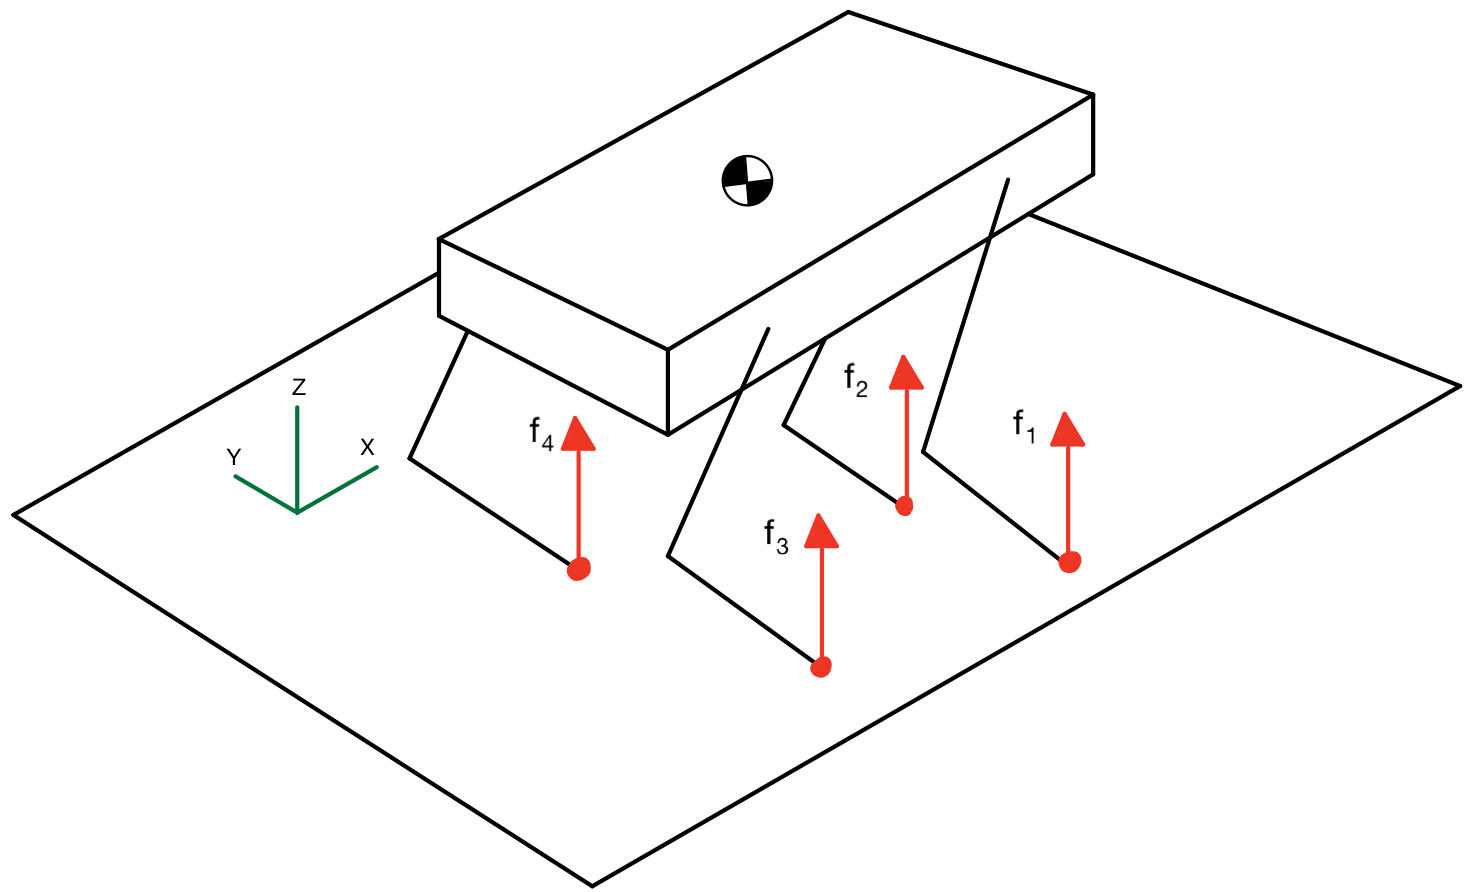
\includegraphics[width=\columnwidth]{altro_mpc/cartoon_quadruped.png}
    \caption{Simplified quadruped model considers a single rigid body that neglects the inertia of the legs. Approximate Newton-Euler equations are defined with leg forces acting at the foot contacts.}
    \label{fig:quad_cartoon}
\end{figure}

Based on \cite{carlo_Dynamic_2018}, we model the robot as a single rigid body with
with $x_k \in \R^{12}$ and contact forces acting at the legs treated as
control inputs $u_k \in \R^{12}$.
A convex problem is obtained by linearizing the dynamics about the current
reference, resulting in a problem similar to \eqref{opt:random_linear}, but
with additional friction-cone constraints on the foot contact forces,
\begin{subequations}
\begin{align}
    \norm{f_{i,k}^t}_2 &\leq \mu f_{i,k}^n  && i \in \{1,\hdots,4\} ,\label{eq:quad_friction} \\
    0 &\leq f_{i,k}^n && i \in \{1, \hdots, 4\}
\end{align}
\end{subequations}
where $f_{i,k}^t$ and $f_{i,k}^n \in \R^{3}$ are the tangential and normal
components of the contact forces of foot $i$ at time step $k$, respectively.
Most MPC implementations further linearize the second-order friction cone
constraint \eqref{eq:quad_friction},
\begin{equation}
\begin{aligned}
    -\tilde{\mu} f^{n} &\leq f^{t_x} \leq \tilde{\mu} f^{n} ,\\ 
    -\tilde{\mu} f^{n} &\leq f^{t_y} \leq \tilde{\mu} f^{n} ,\\ 
    % 0 &\leq f^{n}
\end{aligned}
\end{equation}
resulting in a QP. Both the original SOCP and linearized QP versions of the
problem can be solved with ALTRO-C.

ALTRO-C was compared to OSQP using the QP formulation and ECOS for the SOCP
formulation. The MuJoCo simulator \cite{todorov_MuJoCo_2012} was used to
simulate the full nonlinear dynamics of the quadruped walking in place.
ALTRO-C and OSQP were warm started with the solution from the previous step.
Timing results are shown in Fig. \ref{fig:quad_timing}. While OSQP is
slightly faster than ALTRO-C, both solvers achieve sub-millisecond times.
Interestingly, ALTRO-C achieves nearly the same solve time on the SOCP
formulation, while ECOS is many times slower. This result demonstrates that
the common practice of linearizing friction cones to achieve faster MPC solve
times may be unnecessary with better-optimized solvers.

Finally, we note that non-convex versions of this problem have also been
successfully demonstrated using the IPOPT solver
\cite{bledt_Implementing_2019}. Because ALTRO is a general nonlinear solver,
it can also seamlessly handle such non-convex extensions without having to
change solvers, and while maintaining high performance.

\begin{figure}
    \centering
    \includegraphics[width=\columnwidth,height=4cm]{altro_mpc/quadruped_times.tikz}
    \caption{Timing results for the quadruped benchmark averaged over 60 MPC
    iterations. The QP results are for the linearized friction cone, while
    the SOCP results are for the second-order friction cone. Error bars
    denote one standard deviation.}
    \label{fig:quad_timing}
\end{figure}

\subsection{Rocket Soft Landing}
The rocket soft-landing problem involves landing a vehicle on the surface of
a planet while respecting actuator and safety constraints. Several previous
works have formulated this problem as a convex second-order cone program
\cite{acikmese_Convex_2007,blackmore_MinimumLandingError_2010,blackmore_Lossless_2012,acikmese_Lossless_2013}
% \cite{Acikmese2007, blackmore_minimum-landing-error_2010, Blackmore2012, Acikmese2013}. 
It is standard to decompose the MPC problem into two separate
controllers: a long-horizon controller for the translation dynamics, and a
short-horizon attitude controller. Here we consider the translation problem,
adapted from \cite{acikmese_Lossless_2013},
\begin{mini!}[2]
    {X,U}{\sum_{k=1}^N \norm{x_k - \bar{x}_k}^2_{Q_k} + \sum_{k=1}^{N-1} \norm{u_k}^2_{R}}{}{}
    \addConstraint{x_{k+1}}{= A x_k + B u_k + b}
    \addConstraint{x_1}{= x_{init}}
    \addConstraint{\norm{u_k}_2}{\leq u_{max}} \label{eq:rocket_maxthrust} 
    \addConstraint{\norm{[u_{k, x}\; u_{k,y}]^T}_2}{\leq \alpha_u u_{k, z}} \label{eq:rocket_thrustangle}
    \addConstraint{\norm{[x_{k, x}\; y_{k,y}]^T}_2}{\leq \alpha_x x_{k, z}} \label{eq:rocket_glideslope}
    % \label{eq:rocket_landing}
\end{mini!}
where $x_k \in \R^{6}, u_k \in \R^{3} = \begin{bmatrix} u_{k,x} & u_{k,y} &
u_{k,z} \end{bmatrix}^T$, and the dynamics are approximated by a point mass
subject to gravity.
% \begin{equation}j
%     A = \begin{bmatrix} 0 & I \\ -(\skewmat{\omega})^2 & -2\skewmat{\omega} \end{bmatrix} \quad B = \begin{bmatrix} 0 \\ \frac{1}{m} I \end{bmatrix} \quad b = \begin{bmatrix} 0 \\ g \end{bmatrix} \label{eq:rocket_dynamics}
% \end{equation}
% where $\omega$ is the angular velocity of the planet or moon and $g$ is the acceleration due to gravity. 
The three second-order cone constraints \eqref{eq:rocket_maxthrust},
\eqref{eq:rocket_thrustangle}, and \eqref{eq:rocket_glideslope} enforce a
maximum thrust, thrust angle, and a safe glideslope region, respectively.

To highlight the advantage of handling second-order cone constraints
in ALTRO-C, we optimized the 15 second, 301 knot point reference trajectory
with both ALTRO and ALTRO-C, each to a constraint tolerance of $10^{-5}$.
Since only ALTRO-C handles conic constraints directly, ALTRO enforced the
squared version of Eq.
\eqref{eq:rocket_maxthrust}-\eqref{eq:rocket_glideslope} at each time step.
ALTRO-C took a median time of 25.4 ms and 24 iterations, while the original
version of ALTRO took 40.0 ms and 76 iterations.

For the convex MPC problem with a horizon length of 20 time steps,
ALTRO-C was roughly ten times faster than ECOS, converging in under 4
iterations and 0.37 $\pm$ 0.33 ms, compared to 3.80 $\pm$ 0.18 ms for ECOS.
Fig. \ref{fig:tol_comp} highlights the convergence characteristics of ALTRO-C
compared to several other state-of-the-art conic solvers. A reference
``ground-truth'' solution was generated using COSMO \cite{garstka_COSMO_2019}
with very tight tolerances, and the distance to the ground-truth solution was
computed for decreasing solver tolerances. As shown, ALTRO-C converges
extremely quickly to a solution very close to the true solution, while other
solvers require much tighter tolerances (implying longer solve times) to
achieve similar results.

\begin{figure}
    \centering
    \includegraphics[width=\columnwidth,height=5cm]{altro_mpc/rocket_solver_tol.tikz}
    \caption{Convergence comparison for conic solvers. The error relative to
    a reference trajectory is shown as a function of solver tolerance.}
    \label{fig:tol_comp}
\end{figure}

\subsection{Grasp Optimization}
Grasp optimization for robotic manipulators can be formulated as an SOCP \cite{lobo_Applications_1998}.
%In this prior work, contact forces from the gripper are optimized for a stable grasp at a single moment in time.
We model a two-finger robotic manipulator grasping a box and tracking a
reference trajectory. The box is subject to contact forces from the gripper
$F^1$ and $F^2 \in \R^{3}$, and gravity $F_g$. The inward pointing normal $v^i$
for the $i^{th}$ contact point is useful for separating the contact forces
into the tangential and normal components. The problem setup is illustrated
in Fig. \ref{fig:grasp_fbd_traj}.

\begin{figure}[btp]
    \centering
    \includegraphics[width=\columnwidth,height=7cm]{altro_mpc/grasp_traj.tikz}
    \caption{A free-body diagram and trajectory snapshots for a manipulation
    task. $F^1$ and $F^2$ are the contact forces from the gripper, and $v^i$
    is the inward pointing normal for the object at the $i^{th}$ contact
    point. $F_g$ is the gravitational force. The object pose is shown in
    blue, contact forces are shown in red, and the gravity vector is in
    green. Snapshots that are more transparent correspond to earlier time
    steps in the trajectory.}
    \label{fig:grasp_fbd_traj}
\end{figure}

Similar to \eqref{opt:random_linear}, a quadratic cost function is used to
penalize distance from a reference trajectory. Contact forces are treated as
control inputs, and are subject to the following constraints:
\begin{subequations}
\begin{align}
    &\norm{(I-v_k ^i(v_k ^i)^T) F_k^i}_2\leq \mu (v_k ^i) ^T F_k^i, \quad i = 1,2 \label{eq:grasp_friction} \\
    &(v_k ^i) ^T F_k^i \leq f_{max}, \quad i = 1,2 \label{eq:max_grasp} \\
    &\alpha_k = C_k u_k. \label{eq:torque_balance}
\end{align}
\end{subequations}
Equation \eqref{eq:grasp_friction} enforces Coulomb friction, where
$\norm{(I-v^i (v^i) ^T) F^i}_2$ is the magnitude of the normal component,
$(v^i) ^T F^i$ is the magnitude of the tangential component, and $\mu$ is the
coefficient of friction. Equation \eqref{eq:max_grasp} bounds the normal
force, and \eqref{eq:torque_balance} ensures that the torques generate the
pre-specified reference angular acceleration $\alpha_k \in \R^{3}$.

To ease visualization, the reference trajectory in Fig.
\ref{fig:grasp_fbd_traj} was kept planar, but could easily be extended to 3D.
The performance of ALTRO-C was compared to several other conic solvers for
different MPC horizon lengths $N$. As shown in Fig. \ref{fig:grasp}, while
all solvers exhibit linear scaling with respect to $N$, ALTRO-C exhibits the
fastest run-times---averaging 0.24 ms for 11 knot points and 1.0 ms for 51
knot points.

\begin{figure}[btp]
    \centering
    \includegraphics[width=.75\textwidth,height=6cm]{altro_mpc/grasp_horizon_comp.tikz}
    \caption{Computation time comparison for the grasp optimization MPC
    problem. The solid lines represent average run-time, while the dotted
    lines represent the 1st and 3rd quartiles.}
    \label{fig:grasp}
\end{figure}

\section{Conclusion}
We have presented ALTRO-C, a conic augmented Lagrangian method for solving
model-predictive control problems with general convex conic constraints. The
method was implemented by modifying the open-source ALTRO solver and
demonstrated on several benchmark control problems. ALTRO-C fully exploits
the structure of trajectory optimization problems, achieves fast convergence
to moderate tolerances, and offers good warm-starting capabilities, making it
ideal for MPC applications. Comparisons to several QP and SOCP solvers show
that our algorithm delivers state-of-the-art performance on
small-to-medium-size MPC problems and is suitable for many real-time control
applications. Additionally, unlike other specialized conic solvers, ALTRO-C
can be readily applied to nonlinear and non-convex problems.

Future work will investigate extending ALTRO-C to work with additional cones,
including the semi-definite cone. Further benchmarking results against other
state-of-the-art MPC solvers, such as the newly released HPIPM
\cite{frison_HPIPM_2020}, are also left for future work. While the current
Julia implementation offers significant benefits, a lightweight C
implementation of the algorithm could also be useful for resource-constrained
embedded applications.

\end{document}